\chapter{Conclusion}
\label{sec:conclusion}

\section{Global Interpretations of Results}

The analyses presented in Chapters~\ref{sec:bsm_H_to_tau_tau_analysis} and \ref{sec:H_A_to_4_tau_analysis}, although motivated by different physics, are complementary to one another in context of the type X 2HDM.
The limits on this phase space from the analysis discussed in Chapter~\ref{sec:bsm_H_to_tau_tau_analysis}, are studied using the \textsc{HiggsTools-1} framework~\cite{}.
\textsc{HiggsTools} is a combination of the \textsc{HiggsBounds}, \textsc{HiggsSignals} and \textsc{HiggsPredictions} frameworks and these are used for the following purpose:

\begin{itemize}
\item \textsc{HiggsPredictions} is used to determine theory production cross sections and decay rates.
\item \textsc{HiggsBounds} is used to find direct bounds for searches for new particles.
\item \textsc{HiggsSignals} is used to find the bounds from shifts to the observed Higgs boson's properties.
\end{itemize}

\textsc{HiggsBounds} and \textsc{HiggsSignals} contains a database of results from all key measurements from the LHC, LEP and other colliders.
The result from Chapter~\ref{sec:bsm_H_to_tau_tau_analysis} is included in this database.
The widths of additional Higgs bosons and branching fractions calculated with \textsc{2HDECAY} for Chapter~\ref{sec:H_A_to_4_tau_analysis} are utilised for the scan of the type X 2HDM parameter space.
The cross sections used in each analysis scanned over is scaled to that of the model parameters by the \textsc{NeutralEffectiveCouplings} function in \textsc{HiggsPredictions}.
A 95\% CL limit is then tested on each point in the parameter space. \\

In the alignment scenario, the strongest bounds on the type X 2HDM at all mass points tested come from the analysis described in Chapter~\ref{sec:bsm_H_to_tau_tau_analysis}.
The limits determined for the $m_{\phi}$ equal to 100 and 200 GeV scenarios are overlayed onto the limits shown in Figure~\ref{fig:4tau_md}. \\

\begin{figure}[!hbtp]
\centering
    \subfloat[]{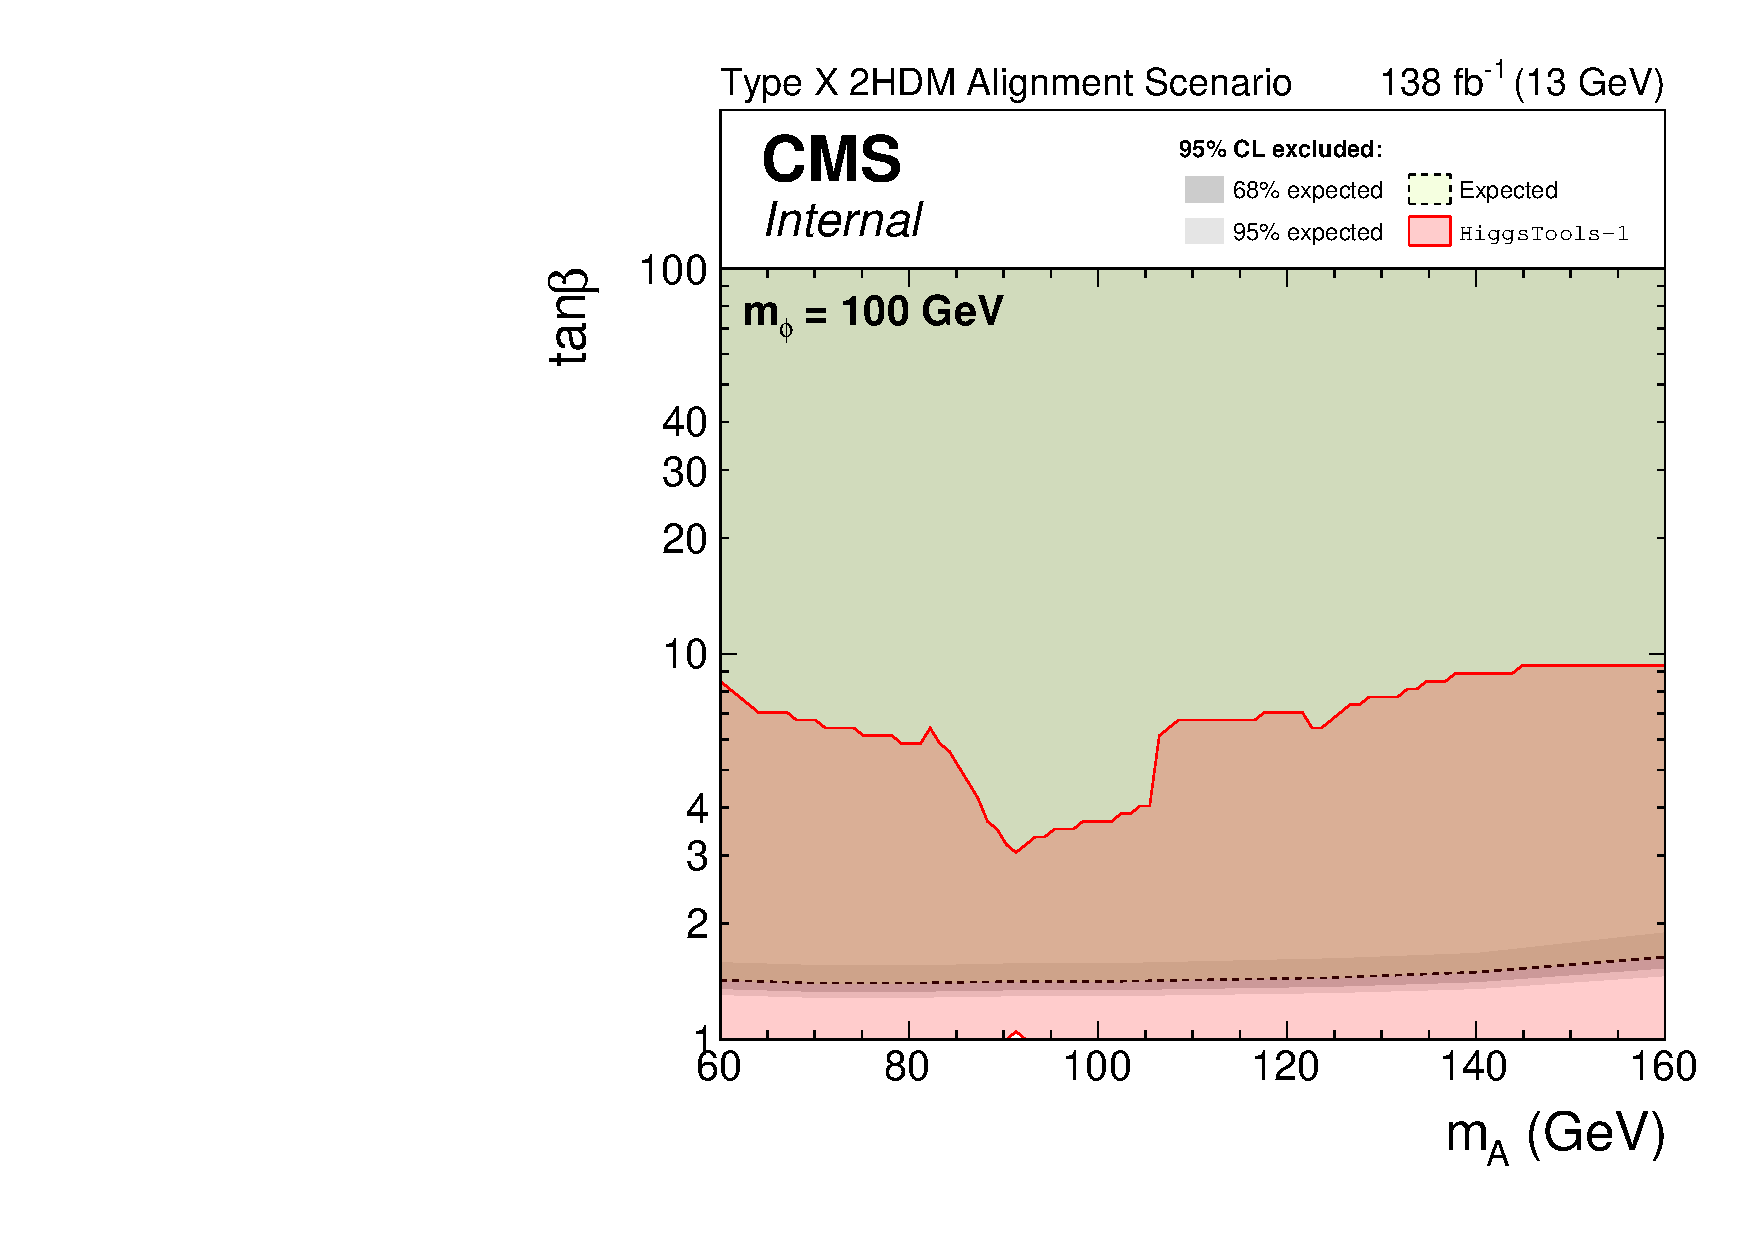
\includegraphics[width=0.7\textwidth]{Figures/md_mphi100_hb.pdf}} \\
    \subfloat[]{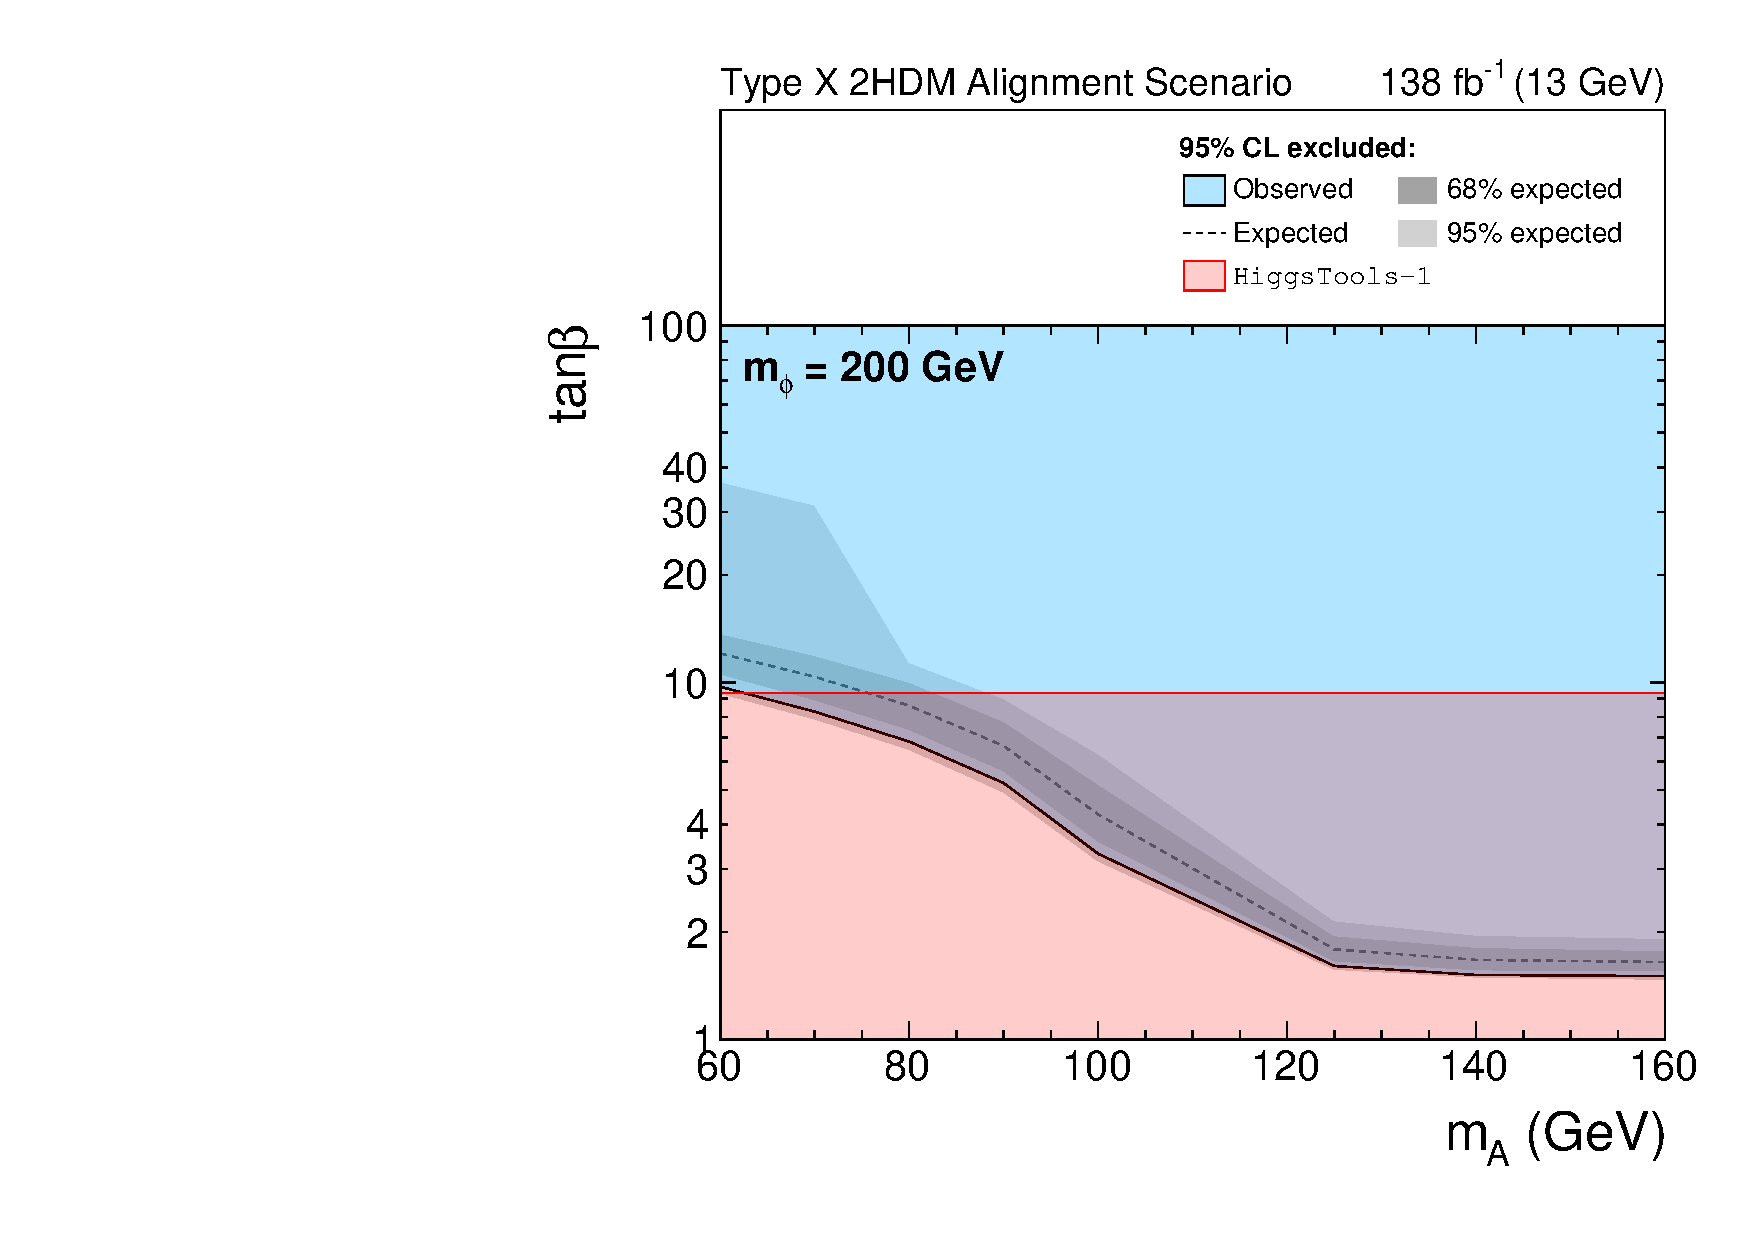
\includegraphics[width=0.7\textwidth]{Figures/md_mphi200_hb.pdf}} 
\caption{Expected and observed 95\% CL exclusion contours on the $m_{A}$-$\tan\beta$ phase space in the type X 2HDM alignment scenario for $m_{\phi}$ scenarios of 100 GeV (a) and 200 GeV (b). The exclusion limit only on background expectation is shown as a dashed black line, the dark and bright grey bands show the 68\% and 95\% intervals of the expected exclusion and the observed exclusion contour is shown by the blue area. The limit obtained by \textsc{HiggsTools} is shown in the red contour.}
\label{fig:4tau_md_hb}
\end{figure}

The type X alignment limit parameter space excluded by Chapter~\ref{sec:bsm_H_to_tau_tau_analysis} comes at low values of $\tan\beta$.
As $\tan\beta$ increases, the gluon fusion and b associated production modes are suppressed but the branching ratios of the additional Higgs bosons to $\tau$ leptons are enhanced.
Therefore, the exclusion limit represents a compromise between suppressed cross sections and enhanced branching ratios. 
The regions where the product is large enough for that parameter point to be excluded, happens at low $\tan\beta$.
In the type X 2HDM, the b associated production mode in negligible due to no enhancement of couplings to b quarks.
The mass hypotheses change the limit due to the non-flat nature of Fig.~\ref{fig:model_independent_limits}(a).
The limit in Fig.~\ref{fig:4tau_md_hb}(b) is flat as the the strongest constraint comes from the $\phi$(H) boson, and for an additional neutral CP-even Higgs boson $\tan\beta \lesssim 10$ is excluded.
However, this is not the case for Fig.~\ref{fig:4tau_md_hb}(a) where $m_{\phi}$ is lighter and the sensitivity is not always driven by the $\phi$(h) boson.
In particular, the limit on a 100 GeV resonance, from Fig.~\ref{fig:model_independent_limits}, is weakest due to the large Drell-Yan background and the local excess observed on top of this peak, and so effects from both additional neutral Higgs bosons are present.
Together, the exclusion limits from both analyses yield an almost complete coverage of the type X 2HDM alignment scenario within the mass range searched. \\

The next question to ask is how the constraints from both BSM searches and precision measurements of the SM Higgs affect the type X 2HDM model, outside of the alignment scenario.
Bounds are again calculated with \textsc{HiggsTools}, however the constraints now come from SM Higgs measurements as well as BSM searches such as described in Chapter~\ref{sec:bsm_H_to_tau_tau_analysis}. \\

OTHER CONSTRAINTS IN THE 2HDM? \\

\section{Outlook}

SUMMARY \\